\documentclass{article}
\usepackage{amsmath,amssymb,enumerate,bbm,calc,capt-of,ifthen}
\usepackage{graphicx}% Include figure files
\usepackage{epsfig}

\newtheorem{cntr}{do not use}
\newcommand{\tmop}[1]{\operatorname{#1}}
\newtheorem{definition}[cntr]{Definition}
\newtheorem{assumption}{Assumption}
\newcommand{\dueto}[1]{\textup{\textbf{(#1) }}}
\newtheorem{varremark}[cntr]{Remark}
\newenvironment{remark}{\begin{varremark}\em}{\em\end{varremark}}
\newcommand{\nin}{\not\in}
\newcommand{\tmem}[1]{{\em #1\/}}
\newtheorem{varnote}{Note}
\newenvironment{note}{\begin{varnote}\em}{\em\end{varnote}}
\newtheorem{proposition}[cntr]{Proposition}

\newenvironment{proof}{
  \noindent\textbf{Proof.}\ }{\hspace*{\fill}
  \begin{math}\Box\end{math}\medskip}

\newenvironment{proofof}[1]{
  \noindent\textbf{Proof of #1.}\ }{\hspace*{\fill}
  \begin{math}\Box\end{math}\medskip}

\newenvironment{proof*}[1]{
  \noindent\textbf{#1\ }}{\hspace*{\fill}
  \begin{math}\Box\end{math}\medskip}

\newtheorem{lemma}[cntr]{Lemma}
\newtheorem{corollary}[cntr]{Corollary}
\newtheorem{theorem}[cntr]{Theorem}
\newenvironment{enumeratenumeric}{\begin{enumerate}[1.]}{\end{enumerate}}
\newtheorem{algo}{Algorithm}

\numberwithin{cntr}{section}
\numberwithin{equation}{section}

\newcommand{\comment}[1]{}
%standard macros
\newcommand{\abs}[1]{\left| #1 \right|}%Absolute value
\newcommand{\absSmall}[1]{| #1 |}%Absolute value, small
\newcommand{\RR}[0]{{\mathbb{R}}}

%Handy macros

\newcommand{\vx}[0]{{\vec{x}}}
\newcommand{\vp}[0]{{\vec{p}}}
\newcommand{\vq}[0]{{\vec{q}}}
\newcommand{\vr}[0]{{\vec{r}}}
\newcommand{\vm}[0]{{\vec{m}}}
\newcommand{\vv}[0]{{\vec{v}}}

\newcommand{\oneto}[1]{{1 \ldots #1}}
\newcommand{\onetoN}[0]{{1 \ldots N}}
\newcommand{\Oto}[1]{{0 \ldots #1-1}}
\newcommand{\OtoN}{{0 \ldots N-1}}

\newcommand{\pointData}{{ \{ \vp_{i} \}_{i=\OtoN} }}
\newcommand{\tanData}{{ \{ \vm_{i} \}_{i=\OtoN} }}

\newcommand{\curveSet}{{ \{ \gamma_i(t) \}_{\Oto{M}}}}
\newcommand{\poly}{{\Gamma}}

\newcommand{\ball}[2]{ { B_{#1}(#2) } }
\newcommand{\allowed}[2]{ { A_{#1}(#2) } }

\newcommand{\curvemax}{{\kappa_{m}}}
\newcommand{\curvemaxi}{{\curvemax^{-1}}}

\newcommand{\curvesep}{{\delta}}

\begin{document}

\title{Reconstructing Curves from Points and Tangents}

\author{L. Greengard and C. Stucchio}

\maketitle

\begin{abstract}
  Abstract goes here
\end{abstract}

\section{Introduction}

In this work, we consider the problem of reconstructing a $C^{1}$ \emph{figure} -- a family of curves $\curveSet$. The data we are given consists of an unorganized set of points $\pointData$, as well as \emph{unit} tangents to the points $\tanData$. Note that the tangents have no particular orientation; making the change $m_{i} \rightarrow -m_{i}$ destroys no information.

Our goal in this work is to construct an algorithm which reconstructs the polygonalization of the curve from this data. An example of a polygonalization is given in Figure \ref{fig:polygonalization}.

\begin{definition}
  \label{def:polygonalization}
  A polygonalization of a figure $\curveSet$ is a planar graph $(V,E)$ with the property that each vertex $p \in V$ is a point on some $\gamma_{i}(t)$, and each edge connects points which are adjacent samples of some curve $\gamma_{i}$.
\end{definition}

\begin{figure}
\setlength{\unitlength}{0.240900pt}
\ifx\plotpoint\undefined\newsavebox{\plotpoint}\fi
\sbox{\plotpoint}{\rule[-0.200pt]{0.400pt}{0.400pt}}%
\includegraphics[scale=0.5]{polygonalization_example.eps}

\caption{A figure and it's polygonalization, c.f. Definition \ref{def:polygonalization}. }
\label{fig:polygonalization}
\end{figure}

The topic of reconstructing figures solely from point data $\pointData$ has been the subject of considerable attention \cite{amenta98crust,amenta98new,dey99curve,hoppe92surface,amenta02simple, dey01reconstructing}. This is actually a more difficult problem, and only weaker results are possible. The main difficulty is the following; if the distance between two separate curves $\gamma_{i}$ and $\gamma_{j}$ is smaller than the sample spacing, then it is difficult to determine which points are associated to which curve. Thus, sample spacing must be $O(\curvesep)$, with $\curvesep$ the distance between different curves.

Tangential information makes this task easier; if two points are nearby (say $\vp_{1}$ and $\vp_{2}$), but $\pm \vm_{1}$ does not point (roughly) in the direction $\vp_{2}-\vp_{1}$, then $\vp_{1}$ and $\vp_{2}$ should not be connected. This fact allows us to reduce the sample spacing to $O(\curvesep^{1/2})$, rather than $O(\curvesep)$. This is to be expected; knowledge of a function and it's derivatives allows interpolation with quadratic accuracy.

In this work, we present an algorithm which allows us to reconstruct a curve from $\pointData$ and $\tanData$. We make two assumptions, under which the algorithm is provably correct.

\begin{assumption}
  \label{ass:curvature}
  We assume each curve $\gamma_{i}$ has bounded curvature:
  \begin{equation}
    \label{eq:curvatureAssumption}
    \forall i = \Oto{M}, ~ \frac{
      \abs{\gamma_{i,x}'(t) \gamma_{i,y}''(t) - \gamma_{i,y}'(t) \gamma_{i,x}''(t)}
    } {
      (\gamma_{i,x}'(t)^{2}+\gamma_{i,y}'(t)^{2})^{3/2}
    } \leq \curvemax
  \end{equation}
\end{assumption}

This assumption is necessary to prevent the curves from oscillating too much between samples.

\begin{assumption}
  \label{ass:separation}
  We assume the curves $\gamma_{i}$ and $\gamma_{j}$ are uniformly separated from each other, i.e.:
  \begin{subequations}
    \begin{equation}
      \label{eq:separationAssumption}
      \sup_{t,t'} \abs{ \gamma_{i}(t) - \gamma_{j}(t')} \geq \curvesep \textrm{~for~} i \neq j
    \end{equation}
    We also assume different areas of the same curve are separated
    from each other:
    \begin{equation}
      \label{eq:separationAssumptionSameCurve}
      \sup_{\abs{t-t'} > \curvemaxi\pi/2 } \abs{ \gamma_{i}(t) - \gamma_{i}(t')} \geq \curvesep
    \end{equation}
  \end{subequations}
  (assuming the curve $\gamma_{i}(t)$ proceeds with unit speed).
\end{assumption}

This assumption makes sure the curves do not come too close together for us to determine which points correspond to which curve (or which part of the same curve). This is illustrated in Figure \ref{fig:separationBetweenCurves}.

\begin{figure}
\setlength{\unitlength}{0.240900pt}
\ifx\plotpoint\undefined\newsavebox{\plotpoint}\fi
\sbox{\plotpoint}{\rule[-0.200pt]{0.400pt}{0.400pt}}%
\includegraphics[scale=0.5]{assumption_two.eps}

\caption{An illustration of Assumption \ref{ass:separation}. The black arrow illustrates \eqref{eq:separationAssumption}, while the red arrow illustrates \eqref{eq:separationAssumptionSameCurve}.}
\label{fig:separationBetweenCurves}
\end{figure}

\section{Geometry}
\subsection{Definition and notations}
Before we begin, we define some notation which we will use.

\begin{definition}
  \label{def:perp}
  For a vector $\vv$, let $\vv^{\perp}$ denote the vector $\vv$ rotated $\pi/2$ to the right.
\end{definition}

\begin{definition}
  \label{def:metric}
  Let $d(\vp,\vq)$ denote the usual Euclidean metric, $d(\vp,\vq) = \abs{\vp - \vq}$. Let $d_{\vm}(\vp,\vq)$ denote the distance in the $\vm$ direction between $\vp$ and $\vq$, i.e. $d_{\vm}(\vp,\vq) = \abs{ (\vp - \vq) \cdot \vm}$.
\end{definition}

\begin{definition}
  For a point $\vp$ and a curve $\gamma_{i}(t)$, we say that $\vp \in \gamma_{i}(t)$ if $\exists t, \gamma_{i}(t)=\vp$.
\end{definition}

As is normal for most interpolation theorems, we need an assumption on the variation of the curve, in this case the curvature.

\subsection{The Algorithm}

We assume there is a set of curves $\curveSet$, which we call the figure. Our goal is to construct a polygonalization of $\curveSet$ from data consisting of points $\pointData$ and tangent directions at the points, $\tanData$. Before we explain the algorithm that calculates the polygonalization, we prove a basic lemma which forms the foundation of our method.
\begin{lemma}
  \label{lem:forbiddenZone}
  For every $i \neq j$, if $\vp_{j} \in \ball{\curvemaxi}{\vp_{i} \pm \vm_{i}^{\perp} \curvemaxi}$, then $(\vp_{i},\vp_{j})$ is not an edge in $\poly$. Here, $\ball{r}{\vp}$ is the ball of radius $r$ about $\vp$.

  We refer to the set $\cup_{\pm} \ball{\curvemaxi}{\vp_{i} \pm \vm_{i}^{\perp} \curvemaxi}$ as the \emph{forbidden zone}; this region is illustrated in Fig. \ref{fig:forbiddenZone}.
\end{lemma}
\begin{figure}
\setlength{\unitlength}{0.240900pt}
\ifx\plotpoint\undefined\newsavebox{\plotpoint}\fi
\sbox{\plotpoint}{\rule[-0.200pt]{0.400pt}{0.400pt}}%
\includegraphics[scale=0.5]{forbidden_zone.eps}

\caption{The forbidden zones, as described in Lemma \ref{lem:forbiddenZone}. The pink is the forbidden zone, and the blue is the set of points a distance $\pi \curvemaxi/2$ away from $p_{i}$.}
\label{fig:forbiddenZone}
\end{figure}
\begin{proof}
  Suppose for simplicity that $\vp_{i}=(0,0)$ and $\vm_{i}=(1,0)$. Now, consider a line $\tau(t)$ of maximal curvature. The curve of maximal curvature, with $\tau_{y}'(t) > 0$ and proceeding at speed $\curvemaxi$ is $\tau^{+}(t)=(\curvemaxi \sin(t), \curvemaxi (1-\cos(t)))$, while the curve with $\tau_{y}'(t) < 0$ is $\tau^{-}(t)=(\curvemaxi \sin(t), \curvemaxi (\cos(t)-1))$.

Any other curve $\gamma(t)$ must lie between these curves (the blue and green curves in Fig \ref{lem:forbiddenZone}). Thus, it is confined to the blue region while it's arc length is less than $\curvemaxi \pi/2$. If $\gamma(t)$ connects $\vp_{i}$ to $\vp_{j}$, then it must do so after travelling a distance greater than $\curvemaxi \pi/2$.

\end{proof}

This shows that the extra information the tangents provides us can be used to exclude certain edges from the polygonalization; basically, all edges should point roughly in the direction of the tangent. This allows us to reject edges which would point in the wrong direction, yielding a more accurate polygonalization (c.f. Fig. \ref{fig:proximityVsTangentBased}).

\begin{figure}
\setlength{\unitlength}{0.240900pt}
\ifx\plotpoint\undefined\newsavebox{\plotpoint}\fi
\sbox{\plotpoint}{\rule[-0.200pt]{0.400pt}{0.400pt}}%
\includegraphics[scale=0.5]{tangents_good_for.eps}

\caption{A naive proximity-based reconstruction algorithm (shown), or even $\beta$-crust type algorithms, will add edges between different curves. Knowledge of the forbidden zone (indicated in pink) allows us to remove such edges.}
\label{fig:proximityVsTangentBased}
\end{figure}

\begin{definition}
  Define the set $\allowed{\epsilon}{\vp}$ to be:
  \begin{equation}
    \label{eq:allowedRegion}
    \allowed{\epsilon}{\vp}=\ball{\epsilon}{\vp_{i}} \setminus \left[ \cup_{\pm} \ball{\curvemaxi}{\vp_{i} \pm \vm_{i}^{\perp} \curvemaxi} \right]
  \end{equation}
  That is, $\allowed{\epsilon}{\vp}$ is the ball of radius $\epsilon$ about $p$ excluding the forbidden zone.  We call this the \emph{allowed zone} or \emph{allowed region}.
\end{definition}
Any edge in the polygonalization starting at $\vp$, with length shorter than $\epsilon$, must connect to another point $\vq \in \allowed{\epsilon}{\vp}$.

We are now ready to describe the polygonalization algorithm.

\begin{algo}
  \label{algo:polygonalization}
  {\bf Polygonalization Algorithm }

  { \bf Input: }

  \begin{itemize}
  \item The maximal curvature, $\curvemax$.
  \item A parameter $\epsilon$ satisfying $\epsilon \curvemax < 2^{-1/2}$ and $2 \curvemax \epsilon^{2} < \curvesep$.
  \item The data $\pointData$ and $\tanData$. We assume that points adjacent on a given curve have a distance shorter than $\epsilon$ between them, i.e. the curve is $\epsilon$-sampled.
  \end{itemize}


  {\bf Algorithm: }

  \begin{enumerate}
  \item Compute the graph $G = (\pointData, E)$ with edge set:
    \begin{equation*}
      E = \{ (\vp_{i},\vp_{j}) : \vp_{i} \in \allowed{\epsilon}{\vp_{j}} \textrm{~and~} \vp_{j} \in \allowed{\epsilon}{\vp_{i}}\}
    \end{equation*}
  \item For each vertex $\vp_{i} \in \pointData$:
    \begin{enumerate}[a.]
    \item Compute the set of vertices
      \begin{equation*}
        R^{\pm}_{i} = \{ \vp_{j} : (\vp_{i}, \vp_{j}) \in E \textrm{~and~} \pm (\vp_{j}-\vp_{i}) \cdot \vm_{i} > 0 \}
      \end{equation*}
    \item Find the nearest tangential neighbors, i.e.
      \begin{equation*}
        \vr^{\pm}_{i} = \textrm{argmin}_{\vq \in R^{\pm}_{i}} d_{\vm_{i}}(\vq, \vp_{i})
      \end{equation*}
    \end{enumerate}
  \item Output the graph $\Gamma = ( \pointData, E')$ with
    \begin{equation*}
      E' = \{ (\vp_{i}, \vr^{+}_{i}) \} \cup \{ (\vp_{i}, \vr^{-}_{i}) \}
    \end{equation*}
    This graph is the polygonalization of $\curveSet$.
  \end{enumerate}

\end{algo}

We also have the following result, which guarantees the correctness of Algorithm \ref{algo:polygonalization}.

\begin{theorem}
  \label{thm:proofOfAlgo}
  Suppose that:
  \begin{subequations}
    \label{eq:separationCondition}
    \begin{equation}
      \delta > 2\curvemax \epsilon^{2}
    \end{equation}
    where $\curvesep$ is as in Assumption \ref{ass:separation} and also
    \begin{equation}
      \label{eq:constraintOnkmaxEpsilon}
      \epsilon < \frac{1}{ \curvemax \sqrt{2}}
    \end{equation}
  \end{subequations}
  Suppose also that the distance between adjacent samples in the polygonalization is bounded by $\epsilon$, i.e. the curve is $\epsilon$-sampled. Then graph $\Gamma$ returned by Algorithm \ref{algo:polygonalization} is the polygonalization of $\curveSet$.
\end{theorem}

We prove this shortly.

\subsection{Proof of Theorem \ref{thm:proofOfAlgo}}

\begin{lemma}
  \label{lem:separationAllowedRegions}
  Let $i \neq j$ and let Assumption \ref{ass:separation} hold. Then for all $t, t'$, if \eqref{eq:separationCondition} and \eqref{eq:constraintOnkmaxEpsilon} hold, then
  \begin{equation}
    \label{eq:connectionsBetweenDifferentCurvesNotAllowed}
    \gamma_{j}(t')  \nin  \allowed{\epsilon}{\gamma_{i}(t)}.
  \end{equation}
  Similarly, if $i=j$ and $\abs{t-t'} \geq \curvemax^{-1} \pi/2$, then \eqref{eq:connectionsBetweenDifferentCurvesNotAllowed} holds.
\end{lemma}
\begin{proof}
  Fix $t$, and define $\vp=\gamma_{i}(t)$ and $\vm=\gamma_{i}'(t) / \abs{\gamma_{i}'(t)}$. Define $L$ to be the line segment $L= \{ \vp+\vm \curvemaxi \sin(\theta) : \theta \in [-\arcsin(\epsilon \curvemax),\arcsin(\epsilon \curvemax)] \}$. The boundaries of $\allowed{\epsilon}{\vp}$ are given by
\begin{equation*}
  \vp + \vm \curvemaxi \sin(\theta) \pm \vm^{\perp} \curvemaxi (1-\cos(\theta)).
\end{equation*}
Now, for any $\vq \in \gamma_{i} $ and $\vq \in \allowed{\epsilon}{\vp}$, the distance between $\vq$ and $L$ is the normal distance to $L$. This distance is bounded by:
\begin{multline}
  \label{eq:1}
  d(\vq,L) \leq
  \sup_{\theta} \curvemaxi \abs{(1-\cos(\theta)) }\\
  \leq
  \sup_{\theta} \curvemaxi 2 \sin^{2}(\theta/2) =
  2\curvemaxi \sin^{2}( \arcsin(\epsilon \curvemax)/2)
\end{multline}
The intermediate value theorem implies $\arcsin( x) \leq \arcsin'(\zeta) x=(1-\zeta^{2})^{-1/2} x$ for some $\zeta \in [0,x]$; since $\epsilon \curvemax < 2^{-1/2}$ (by \eqref{eq:constraintOnkmaxEpsilon}), we find that:
\begin{equation*}
  \arcsin(\epsilon \curvemax) \leq (1-(2^{-1/2})^{2})^{-1/2} \curvemax \epsilon = \sqrt{2} \curvemax \epsilon
\end{equation*}
Substituting this into \eqref{eq:1} yields:
\begin{equation}
  \eqref{eq:1} \leq  2 \curvemaxi \sin^{2}( \sqrt{2} \curvemax \epsilon/2) \leq \curvemax \epsilon^{2}
\end{equation}

Thus, the \emph{normal} distance between any point in $\allowed{\epsilon}{\vp}$ and $L$ is $O(\curvemax \epsilon^{2})$.

If $\gamma_{j}(t') \nin L+\vm^{\perp} \RR$, then clearly $\gamma_{j}(t') \nin \allowed{\epsilon}{\gamma_{i}(t)}$ so we assume $\gamma_{j}(t') \in L+\vm^{\perp} \RR$. In this case, $\gamma_{j}(t') = \vp + \vm \curvemaxi \sin(\theta_{0}) + \vm^\perp z$, with $z \in \RR$ the normal (relative to $L$) distance to $L$.

By the second triangle inequality,
\begin{equation*}
  d_{\vm^{\perp}}(\gamma_{j}(t'), L) \geq \abs{d_{\vm^{\perp}}(\gamma_{j}, \gamma_{i}) -  d_{\vm^{\perp}}(\gamma_{i}, L)}
  \geq \delta - \curvemax \epsilon^{2} > \curvemax \epsilon^{2}
\end{equation*}
But this implies that $d(\gamma_{j}(t'), L) \geq d_{\vm^{\perp}}(\gamma_{j}(t'), L) \geq \curvemax \epsilon^{2}$, and thus $\gamma_{j}(t') \nin \allowed{\epsilon}{\vp}$.

The proof when $i=j$ is identical.
\end{proof}

This result shows that the graph $G$, computed in Step 1 of Algorithm \ref{algo:polygonalization}, separates different $\gamma_{i}$ and $\gamma_{j}$ from each other, as well as different parts of the same curve. Thus, after Step 1, we are left with a graph $G$ having edges only between points $\vp_{i}$ and $\vp_{j}$ which are on the same curve $\gamma_{k}$, and which have are separated in $\gamma_{k}$ by an arc length no more than $\curvemaxi \pi/2$.

We now show that $G$ is a superset of the polygonalization.

\begin{proposition}
  Suppose the point data $\pointData$ is $\epsilon$-sampled, i.e. if two points $\vp_{i}$ and $\vp_{j}$ are adjacent on the curve $\gamma_{k}$, then the \emph{arc length} between $\vp_{i}$ and $\vp_{j}$ is bounded by $\epsilon$. Then $G$ contains the polygonalization of $\curveSet$.
\end{proposition}
\begin{proof}
  If the distance between adjacent points $\vp_{i}$ and $\vp_{j}$ is at most $\epsilon$, then $\vp_{j} \in \ball{\epsilon}{\vp_{i}}$. Since the segment of $\gamma_{k}$ between $\vp_{i}$ and $\vp_{j}$ has arc length less than $\epsilon$, $\vp_{j}$ is not in the forbidden zone of $\vp_{i}$ (by the same argument as in Lemma \ref{lem:forbiddenZone}. Thus, $\vp_{j} \in \allowed{\epsilon}{\vp_{i}}$ (and vice versa), and $(\vp_{i},\vp_{j})$ is an edge in $G$.
\end{proof}

We have now shown that $G$ separates distinct curves, and that $G$ contains the polygonalization of $\curveSet$. It remains to show that $\Gamma$ is the polygonalization.

\begin{lemma}
  \label{eq:closestTangentPointInAllowedRegionIsCorrect}
  Fix a point $\vp_{i}=\vp \in \pointData$. Choose a tangent vector $\vm_{0}$ and fix an orientation. Consider the set of points $\vp_{j}$ such that $(\vp, \vp_{j})$ is an edge in $G$ and $(\vp_{j} - \vp) \cdot \vm_{0} > 0$. Suppose also that $\epsilon$ satisfies \eqref{eq:constraintOnkmaxEpsilon}.

  Then only edge in the polygonalization of $\gamma$ is the edge for which $(\vp_{j} - \vp) \cdot \vm_{0}$ is minimal.
\end{lemma}

\begin{remark}
  The minimal edge is the edge $\vr^{+}_{0}$ as computed in Step (2b) of Algorithm \ref{algo:polygonalization}.
\end{remark}

\begin{proof}
  Change coordinates so that $\vm_{0} = (1,0)$, and parameterize $\gamma(t)=(t,w(t))$. This parameterization is valid locally; the conclusion follows immediately if all points $\vp_{j}$ are contained in the region where this parameterization is valid.

  All we need to do is show that this parameterization is valid on a region of size $\epsilon \curvemax$. This can be done as follows. The parameterization breaks down when $w'(t)$ blows up, we need to show that this does not happen before $t=\epsilon$. Plugging this parameterization into the curvature bound \eqref{eq:curvatureAssumption} yields:
  \begin{equation*}
    \frac{ \abs{w''(t)} }{(1+w'(t)^{2})^{3/2}} \leq \curvemax
  \end{equation*}
  Assuming $w''(t)$ is positive, this is a first order nonlinear differential inequality for $w'(t)$. We can integrate both sides (using the hyperbolic trig substitution $w(t)=\sinh(\theta)$ for the left side) to obtain:
  \begin{equation}
    \label{eq:2}
    \frac{w'(t)}{\sqrt{1+w'(t)^{2}}} \leq \curvemax t
  \end{equation}
  Define $f(z)=z/\sqrt{1+z^{2}}$, then $f^{-1}(z)$ is singular only at $z=\pm 1$, and is regular before that. Solving \eqref{eq:2} for $w'(t)$ shows that:
  \begin{equation*}
    w'(t) \leq f^{-1}(\curvemax t)
  \end{equation*}
  implying that $w'(t)$ is finite for $\curvemax t < 1$, or $t < \curvemaxi 1$. Thus, the parameterization is valid for $t < \curvemaxi$.

  Since each point $\vp_{j} \in \allowed{\epsilon}{\vp_{0}}$, and since $\epsilon < 1/\curvemax \sqrt{2}$ (by \eqref{eq:constraintOnkmaxEpsilon}), this in particular implies each point $\vp_{j}$ is in the region where $t < \curvemaxi$.
\end{proof}

Thus, we have shown that the graph $\Gamma$, as computed by Algorithm \ref{algo:polygonalization}, is the polygonalization of $\curveSet$.

\begin{figure}
\setlength{\unitlength}{0.240900pt}
\ifx\plotpoint\undefined\newsavebox{\plotpoint}\fi
\sbox{\plotpoint}{\rule[-0.200pt]{0.400pt}{0.400pt}}%
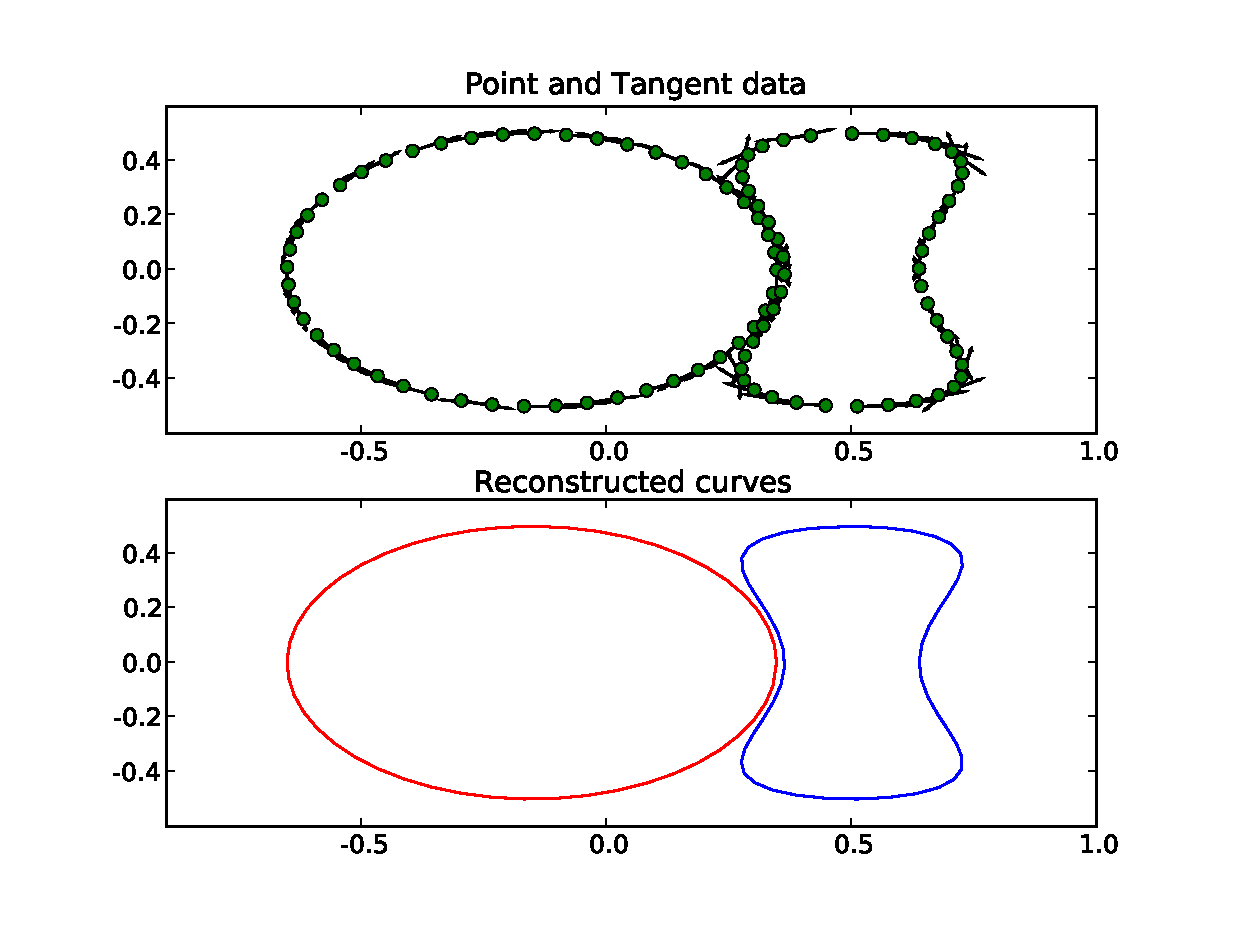
\includegraphics[scale=0.5]{example1.eps}

\caption{Some unordered points/tangents, and the curves reconstructed from them. In this case, $\epsilon=0.065$, $\curvemax=3$ and $\delta=0.015$.}
\label{fig:basicExample}
\end{figure}

\section{Filtering spurious points}

The method provided here is relatively robust with regard to the addition of spurious random data points. This is because spurious data points are highly unlikely to be connected to any other points in the polygonalization graph.

This occurs for two primary reasons. First, for an incorrect data point to be connected to part of the polygonalization at all, it would need to be located in $\allowed{\epsilon}{\vp}$ for some $\vp$. This is a region of length $O(\epsilon)$ and width $O(\epsilon^{2})$. There are approximately $L = \sum_{j} \textrm{arclength}(\gamma_{j})$ such points, for a total volume of $\epsilon^{2} L$. Thus, the probability that a spurious point is in \emph{some} allowed region is roughly $O(L \epsilon^{2})$.

The second reason is that even if a spurious point is in some allowed region, it is unlikely to point in the correct direction. If an erroneous point $\vq$ is inside $\allowed{\epsilon}{\vp}$, it is still not likely that $\vp \in \allowed{\epsilon}{\vq}$; this follows because the tangent at $\vq$ must point in the direction of $\vp$ (with error proportional to $\epsilon^{2}$, the angular width of $\allowed{\epsilon}{\vq}$). Thus, the probability that the tangent at $\vq$ points towards $\vp$ is $O(\epsilon^{2}/2\pi)$.

Based on these arguments, the probability that any \emph{randomly chosen} spurious point $\vq$ is connected to any other point in the polygonalization is $O(L \epsilon^{4})$.

\begin{figure}
\setlength{\unitlength}{0.240900pt}
\ifx\plotpoint\undefined\newsavebox{\plotpoint}\fi
\sbox{\plotpoint}{\rule[-0.200pt]{0.400pt}{0.400pt}}%
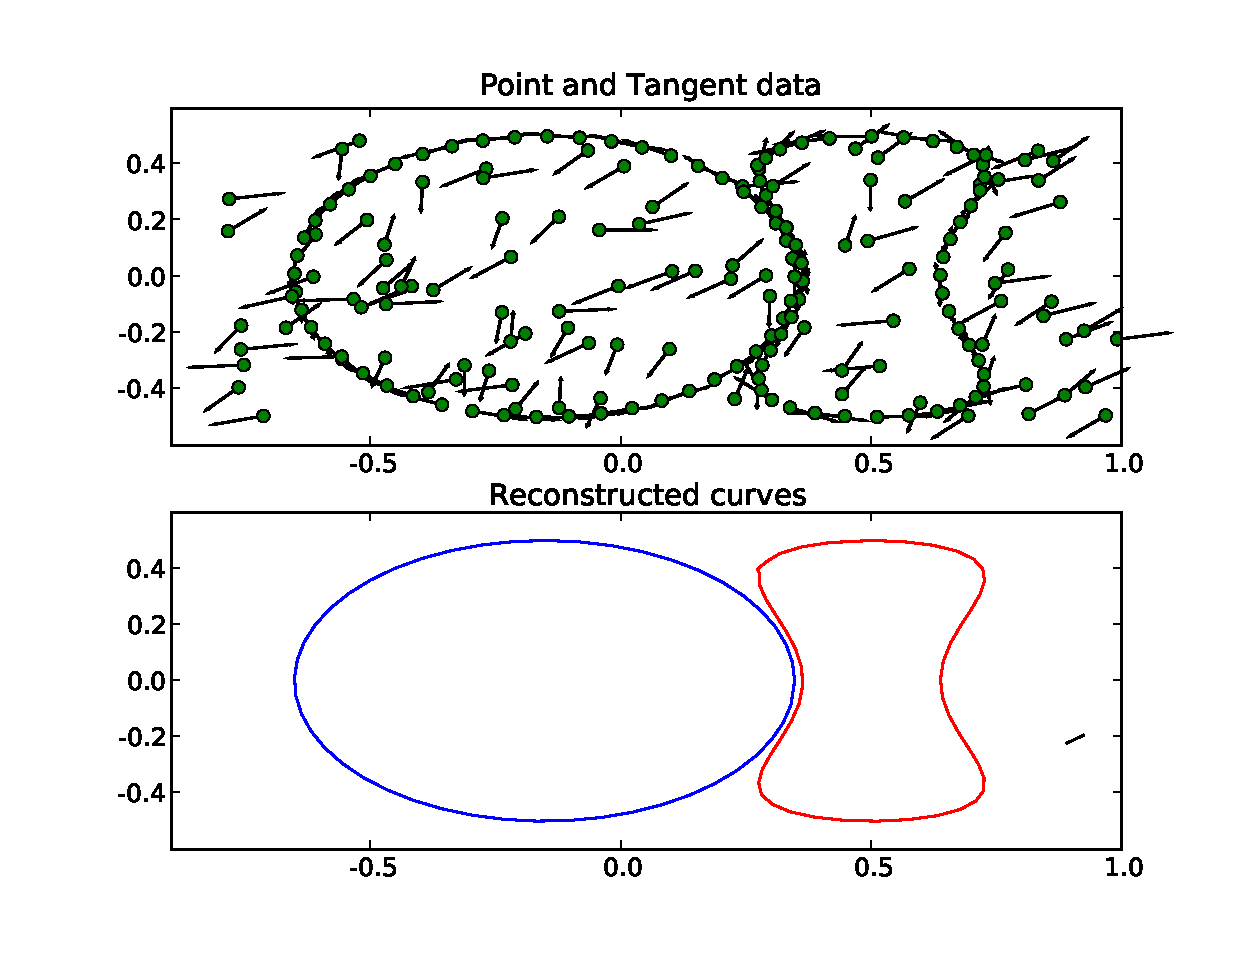
\includegraphics[scale=0.5]{noisy_example.eps}

\caption{The same example as in Figure \ref{fig:basicExample}, but with 100 additional points (for a total of $196$), placed randomly. }
\label{fig:noisyExample}
\end{figure}

\subsection{Noise Removal by Connecting the Dots}

The aforementioned criteria suggest that our ``connect the dots'' algorithm has excellent potential for noise removal. It suggests that if we remove points which do not have edges pointing towards other edges, then with high probability we are removing spurious edges.

In fact, this is born out in practice. By running Algorithm \ref{algo:polygonalization} on a figure consisting of $96$ true points, and $100$ randomly placed incorrect points, a nearly correct polygonalization is calculated; this is shown in Figure \ref{fig:noisyExample}. The original curve is reconstructed with an error at only one point (the top left corner of the red line).

Of course, if enough incorrect points are present, eventually some points will be connected by Algorithm \ref{algo:polygonalization}. This can be seen in Figure \ref{fig:noisyExample}: the black line near $(0.9, -0.2)$ is an edge between two incorrect points. However, spurious edge formations such as this are small in number, and do not usually look like part of the figure.

One hint that an edge is incorrect is if it points to a leaf. That is, consider a set of vertices $\vp_{0}, \vp_{1}, \ldots, \vp_{n}$ as well as $\vq$. Suppose, after approximately computing the polygonalization, one finds that the graph contains edges $e_{0} = (\vp_{0}, \vp_{1}), e_{1} = (\vp_{1}, \vp_{2}), \ldots, e_{n-1} = (\vp_{n-1}, \vp_{n})$ and $e_{n} = (\vp_{n/2}, \vq)$. The vertex $\vq$ is a leaf, i.e. it is reachable by only one edge. A polygonalization should not have leaves, suggesting that the edge $e_{n}$ should not be present. This suggests that by filtering leaves, we can remove primarily noise while leaving the signal undamaged.

An additional problem with noisy data is that sometimes, an incorrect point will be present, in the allowed region of a legitimate point, and closer to the legitimate point than the adjacent points along the curve. This will prevent the correct edge from being added. This can be remedied by adding not only $\vr_{i}^{\pm}$ at Step 3 of the algorithm, but also points for which $d_{\vm^{\perp}}(\vp_{i})$who's distance to $\vp_{i}$ is not much longer than the distance between $\vp_{i}$ and $\vr_{i}^{\pm}$. With some luck, this procedure combined with filtering out leaves will approximately reconstruct the correct figure.

Thus, we arrive at are noisy polygonalization algorithm.

\begin{algo}
  \label{algo:noisyPolygonalization}
  {\bf Polygonalization Algorithm with Noise Removal }

  { \bf Input: }

  \begin{itemize}
  \item The maximal curvature, $\curvemax$.
  \item A parameter $\epsilon$ satisfying $\epsilon \curvemax < 2^{-1/2}$ and $2 \curvemax \epsilon^{2} < \curvesep$.
  \item The data $\pointData$ and $\tanData$, which include spurious data. We assume that points adjacent on a given curve have a distance shorter than $\epsilon$ between them, i.e. the curve is $\epsilon$-sampled.
  \item A leaf removal count, $l \in \mathbb{Z}^{+}$.
  \item A threshold $\alpha \geq 1$.
  \end{itemize}


  {\bf Algorithm: }

  \begin{enumerate}
  \item Compute the graph $G = (\pointData, E)$ with edge set:
    \begin{equation*}
      E = \{ (\vp_{i},\vp_{j}) : \vp_{i} \in \allowed{\epsilon}{\vp_{j}} \textrm{~and~} \vp_{i} \in \allowed{\epsilon}{\vp_{j}}\}
    \end{equation*}
  \item For each vertex $\vp_{i} \in \pointData$:
    \begin{enumerate}[a.]
    \item Compute the set of vertices
      \begin{equation*}
        R^{\pm}_{i} = \{ \vp_{j} : (\vp_{i}, \vp_{j}) \in E \textrm{~and~} \pm (\vp_{j}-\vp_{i}) \cdot \vm_{i} > 0 \}
      \end{equation*}
    \item Find the nearest tangential neighbors, i.e.
      \begin{equation*}
        \vr^{\pm}_{i} = \textrm{argmin}_{\vq \in R^{\pm}_{i}} \pm (\vp_{j}-\vp_{i}) \cdot \vm_{i}
      \end{equation*}
    \item Find the set of almost-nearest tangential neighbors:
      \begin{equation*}
        \mathbf{R}^{\pm}_{i} = \{ \vr \in R^{\pm}_{i} : d_{\vm_{i}}(\vp_{i}, \vr) \leq \alpha \vr^{\pm}_{i} \}
      \end{equation*}
    \end{enumerate}
  \item Compute the graph $\Gamma = ( \pointData, E')$ with
    \begin{equation*}
      E' = \bigcup_{i} \{ (\vp_{i}, \vr) : \vr \in \mathbf{R}^{+}_{i} \} \cup \{ (\vp_{i}, \vr) : \vr \in \mathbf{R}^{-}_{i} \}
    \end{equation*}
  \item Search through $\Gamma$ for leaves, and remove edges pointing to the leaves. Repeat this $l$ times.
  \item Output $\Gamma$.
  \end{enumerate}
\end{algo}

In practice, we have found $\alpha=1.1$ and $l=4$ work reasonably well. Figure \ref{fig:moreNoisyExample} illustrates the result of Algorithm \ref{algo:noisyPolygonalization}, both with and without filtering.

\begin{figure}
\setlength{\unitlength}{0.240900pt}
\ifx\plotpoint\undefined\newsavebox{\plotpoint}\fi
\sbox{\plotpoint}{\rule[-0.200pt]{0.400pt}{0.400pt}}%
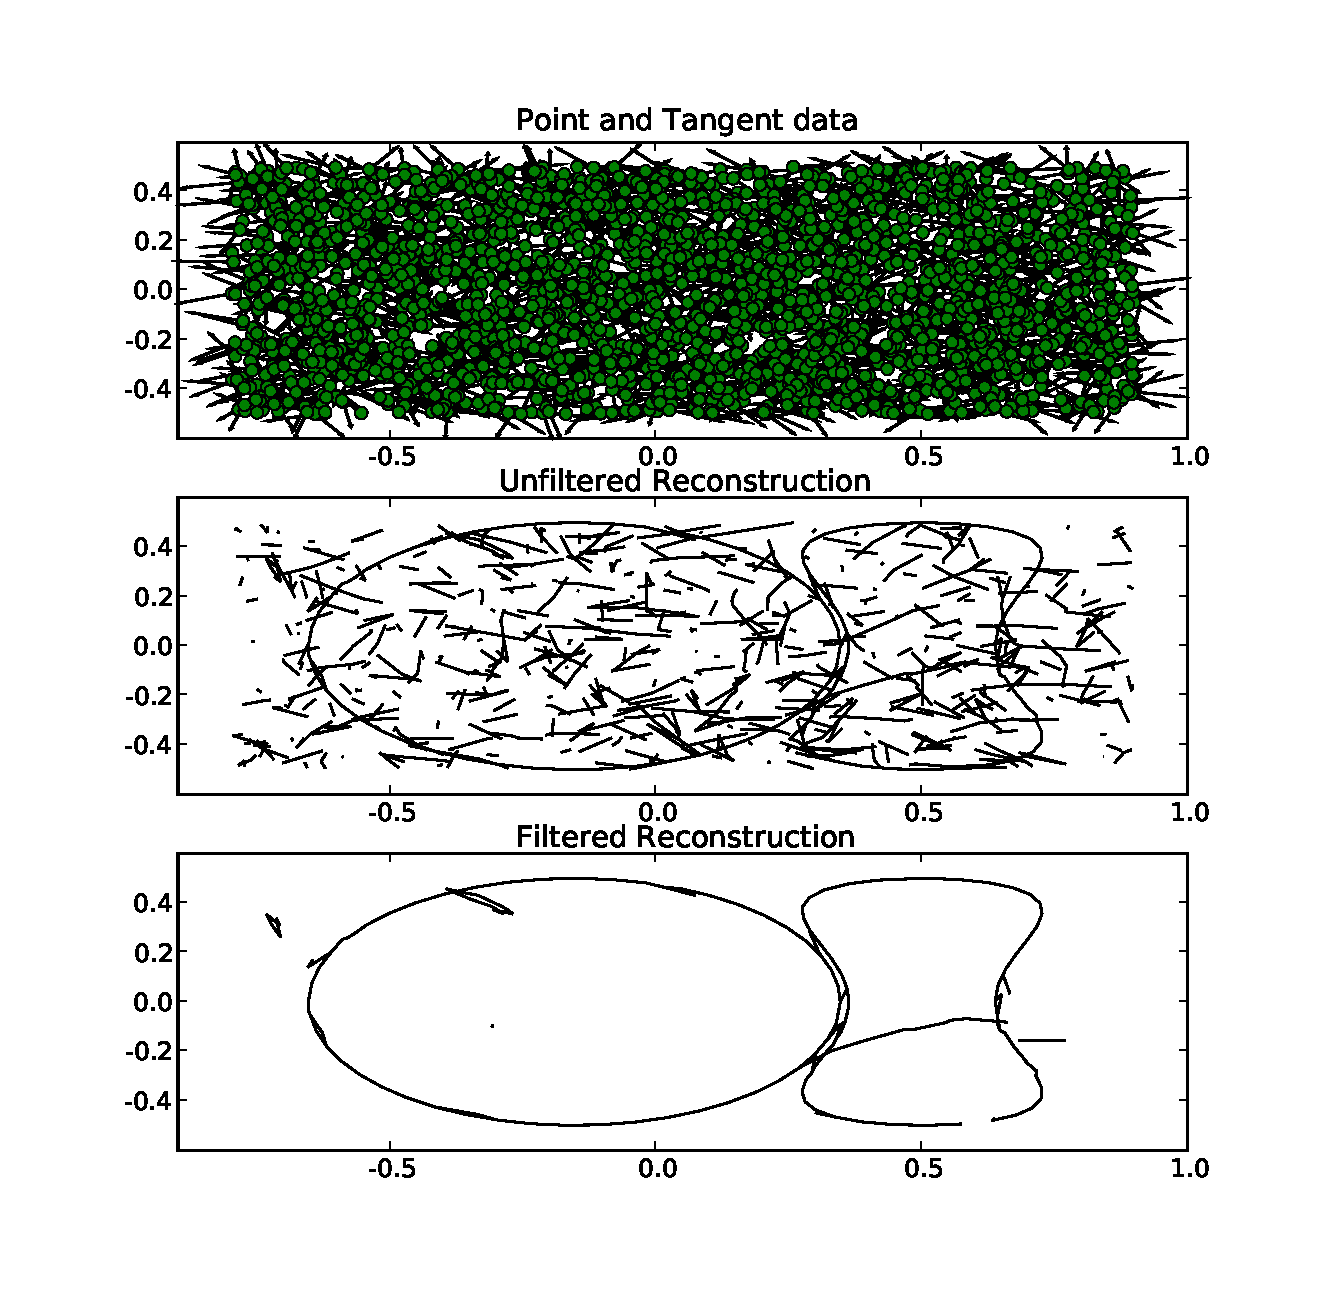
\includegraphics[scale=0.5]{more_noisy_example.eps}

\caption{The same example as in Figure \ref{fig:basicExample}, but with 2000 additional random points added (for a total of 2096). The original curve is no longer completely reconstructed, but the general shape is still roughly visible, along with many more spurious points. Filtering leaves with $l=4$ improves the situation considerably.}
\label{fig:moreNoisyExample}
\end{figure}

\bibliography{../stucchio}
\bibliographystyle{hplain}

\end{document}